% Drawing 146/01-3 -- folder 146, batch 01, archive page 15 (PDF page 16).
% Transcription: une sphère : pôle $P$ en haut et pôle opposé en bas ; l'équateur porte les points $\beta$, $\bar\alpha$ et un troisième point au bord droit ; un parallèle tracé en pointillé porte $\tilde\alpha$, $\alpha$, $\tilde\beta$
% Kind: sphere with marked points. Method 2 (schematic redraw from the facsimile). Status: ok.
% Notes: Equator solid (front half only), dotted parallel above it. The label under the lower pole is not read in the transcription and is left out; the third point at the right end of the equator is unlabelled (its label, if any, is lost in the outline).
% Coordinates: 1 unit = 1 mm = 1/100 of the crop width (bbox in page fractions: [0.1, 0.48, 0.36, 0.64]).
% Redrawn by Claude (claude-opus-5-5), issue #73 pilot, 2026-11-07; not checked by a human; not compiled (no TeX in the session).
% Rights: reproduces part of the work -- behind RENDER_TRANSCRIPTS, never published by itself.
\documentclass[tikz,border=3pt]{standalone}
\usepackage{amsmath,amssymb}
\usetikzlibrary{patterns,arrows.meta}
\tikzset{pencil/.style={black!45}, struck/.style={black!35}, mark/.style={circle,draw,inner sep=1.3pt}, pt/.style={circle,fill,inner sep=0.9pt}, opt/.style={circle,draw,fill=white,inner sep=1.1pt}}
\begin{document}
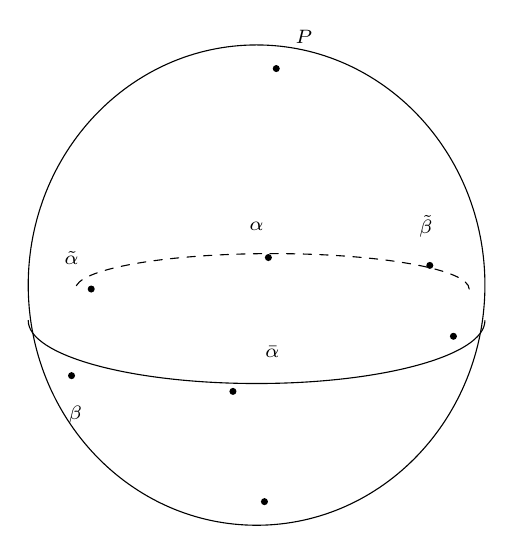
\begin{tikzpicture}[x=1mm,y=1mm,line cap=round,line join=round,font=\scriptsize]
\draw (41,-40.5) ellipse[x radius=29, y radius=30.5];
\draw (12,-45) arc[start angle=180, end angle=360, x radius=29, y radius=8];
\draw[dashed] (68,-41) arc[start angle=0, end angle=180, x radius=25, y radius=4.5];
\node[pt] at (43.5,-13) {};
\node[inner sep=1pt] at (47,-9) {\scriptsize $P$};
\node[pt] at (42,-68) {};
\node[pt] at (17.5,-52) {};
\node[inner sep=1pt] at (18,-57) {\scriptsize $\beta$};
\node[pt] at (38,-54) {};
\node[inner sep=1pt] at (43,-49) {\scriptsize $\bar\alpha$};
\node[pt] at (66,-47) {};
\node[pt] at (20,-41) {};
\node[inner sep=1pt] at (17.5,-37) {\scriptsize $\tilde\alpha$};
\node[pt] at (42.5,-37) {};
\node[inner sep=1pt] at (41,-33) {\scriptsize $\alpha$};
\node[pt] at (63,-38) {};
\node[inner sep=1pt] at (62.5,-33) {\scriptsize $\tilde\beta$};
\end{tikzpicture}
\end{document}
